\section{Results}\label{chap5:results}

Distributions of the \mll and \mt variables after the full analysis selection are shown in Fig.~\ref{fig:mllandmt} for the 0 and 1 jets categories separately, but merging the e$\mu$ and $\mu$e final states together.

\begin{figure}
\centering
\subfigure[0 jets - \mll]{
  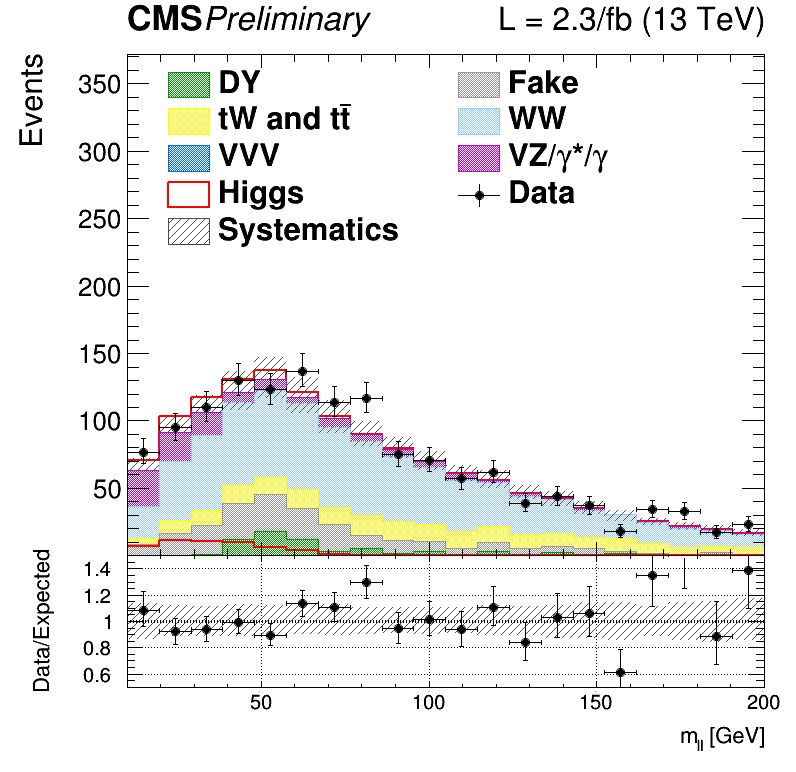
\includegraphics[width=0.45\textwidth]{images/13TeV/cratio_hww2l2v_13TeV_of0j_mll}
}
\subfigure[0 jets - \mt]{
  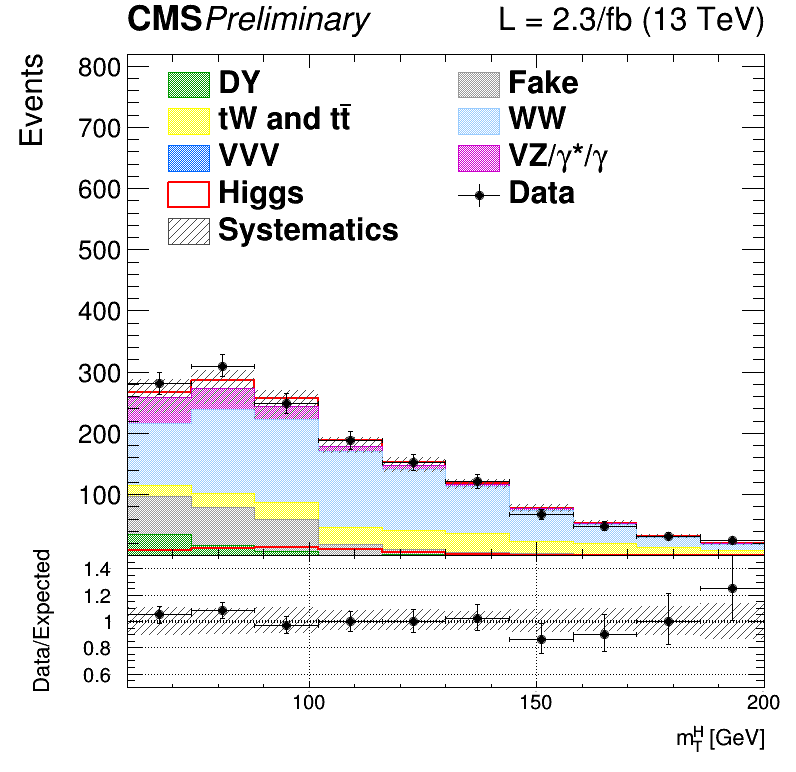
\includegraphics[width=0.45\textwidth]{images/13TeV/cratio_hww2l2v_13TeV_of0j_mth}
}\\
\subfigure[1 jet - \mll]{
  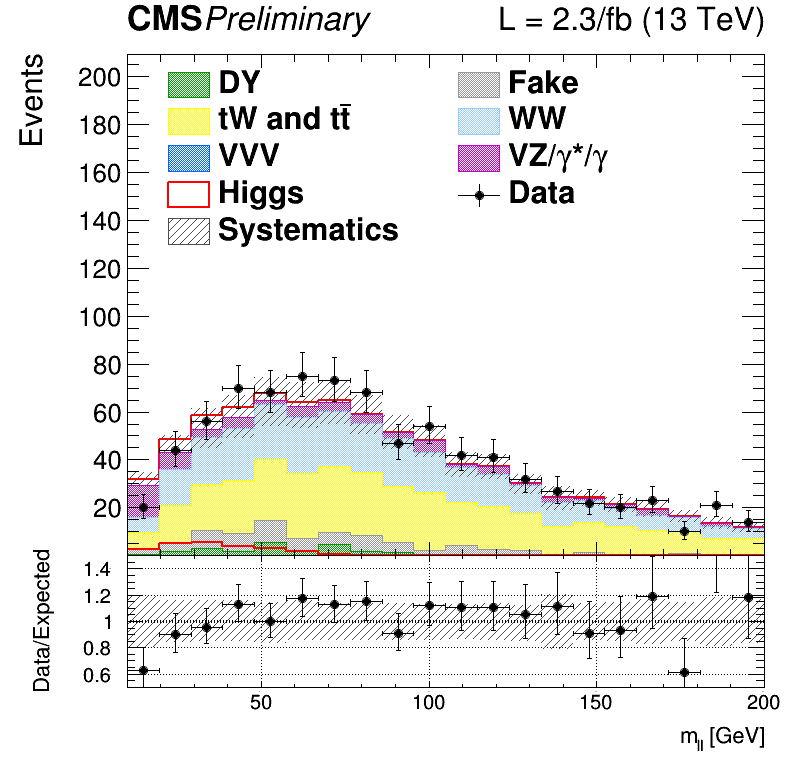
\includegraphics[width=0.45\textwidth]{images/13TeV/cratio_hww2l2v_13TeV_of1j_mll}
}
\subfigure[1 jet - \mt]{
  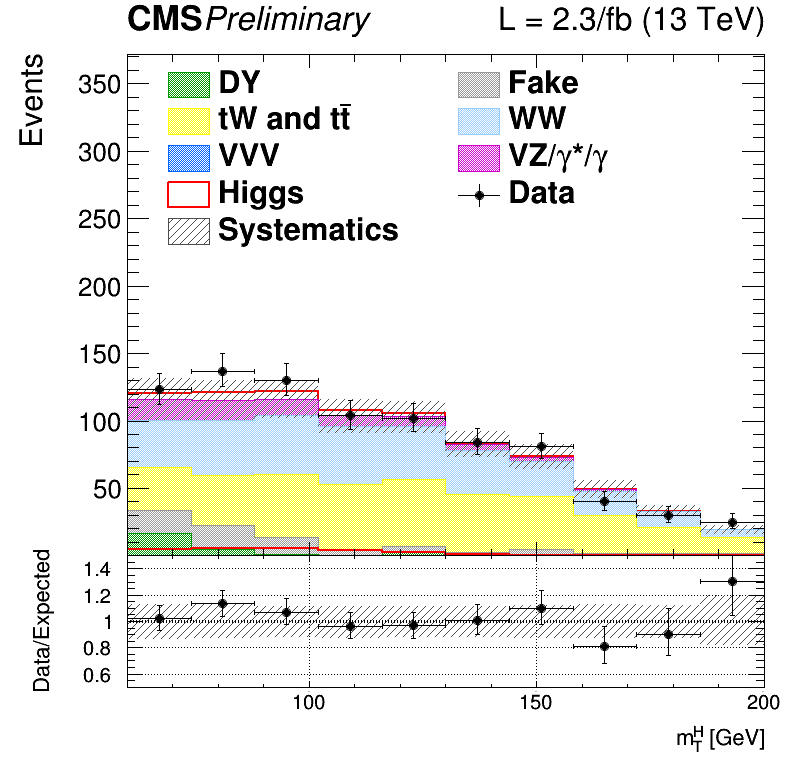
\includegraphics[width=0.45\textwidth]{images/13TeV/cratio_hww2l2v_13TeV_of1j_mth}
}
\caption{Distributions of \mll (left) and \mt (right) for events with 0 jets (upper row) and 1 jet (lower row), for the main backgrounds (stacked histograms), and for a SM Higgs boson signal with $m_\mathrm{H}=125$\GeV (superimposed and stacked red histogram) after the analysis event selections. The simulation of the WW background is normalized to data.}\label{fig:mllandmt}
\end{figure}

The expected and observed signal significances are shown in Table~\ref{tab:13TeVsignif} for all the categories. Also, the observed signal strengths and the corresponding uncertainties are shown. The best fit signal strength obtained combining all the categories together is found to be $0.3^{+0.5}_{-0.5}$, corresponding to an observed significance of $0.7\,\sigma$, to be compared with the expected significance of $2.0\,\sigma$ for a Higgs boson mass of 125\GeV.

The measurement is dominated by the statistical uncertainties in data. The main systematic contributions affecting the uncertainty in the signal strength arise from the Fake background estimation, lepton identification and isolation, luminosity, b tagging scale factors, WW and \ttbar background normalization and other minor backgrounds. The uncertainties in the data driven backgrounds mainly arise from the limited data statistics in the control regions used for measuring the normalization.
A summary of the most important systematic uncertainties and their effect on the signal strength uncertainty is illustrated in Table~\ref{tab:mu_syst}.

\begin{table}[htb]
\caption{Observed and expected significance and signal strength for the SM Higgs boson with $m_{\rm H}=125$\GeV in the 0 and 1 jets categories. The $\mu$e and e$\mu$ configurations are shown separately.}\label{tab:13TeVsignif}
\begin{center}
\begin{tabular}{lccc}
\toprule
Category  &  Expected significance      &  Observed  significance    &  $\sigma/\sigma_{SM}$     \\
\midrule
0 jet  $\mu$e   &     1.1        &  1.3        &  1.13 $_{-0.9}^{+0.9}$             \\ [2pt]
0 jet  e$\mu$   &     1.3        &  0.4        &  0.33 $_{-0.7}^{+0.7}$             \\  [2pt]
1 jet  $\mu$e   &     0.8        &  0          &  -0.11$_{-1.7}^{+0.5}$                 \\[2pt]
1 jet  e$\mu$   &     0.9        &  0          &  -0.54$_{-1.4}^{+1.4}$                 \\ [2pt]
\midrule 
0 jet           &     1.6        &  1.3       &  0.71$_{-0.5}^{+0.6}$             \\  [2pt]
1 jet           &     1.2        &  0         &  -0.56$_{-1.0}^{+1.0}$                \\[2pt]
\midrule 
Combination     &     2.0        &  0.7       &  0.33$_{-0.5}^{+0.5}$              \\[2pt]
\bottomrule
\end{tabular}
\end{center}
\end{table}


\begin{table}[htb]
\caption{Main systematic sources and their contribution to the signal strength uncertainty ($\Delta\mu/\mu$).}\label{tab:mu_syst}
\begin{center}
\begin{tabular}{lc}
\toprule
Systematic uncertainty  &   $\Delta\mu/\mu$\\
\midrule
Fake background estimation & 25\% \\
Lepton identification and isolation & 20\% \\
W$\gamma^*$ background cross section & 12\% \\
WW and \ttbar data driven normalization & 10\% \\
Luminosity & 8\% \\
b tagging scale factors & 6\% \\
Lepton scale and resolution & 3\% \\
\bottomrule
\end{tabular}
\end{center}
\end{table}
